\documentclass[a4paper, 12pt, UTF8]{article}

\usepackage{xeCJK}
% \setCJKmainfont[BoldFont={SimHei},ItalicFont={KaiTi}]{SimSun}
\setCJKmainfont[ItalicFont={AR PL UKai CN}]{AR PL UMing CN}
\setCJKsansfont{WenQuanYi Zen Hei} %设置中文无衬线字体为文泉驿正黑
\setCJKmonofont{WenQuanYi Zen Hei Mono} %设置中文打字机(等宽)字体为文泉驿正黑

\usepackage{amsfonts}
\usepackage{amsmath}
\usepackage{graphicx}
\usepackage{indentfirst}
\usepackage{listings}
\lstset{
    columns=flexible,
    breakatwhitespace=false,
    breaklines=true,
    frame=single,
    numbers=left,
    numbersep=5pt,
    showspaces=false,
    showstringspaces=false,
    showtabs=false,
    stepnumber=1,
    rulecolor=\color{black},
    tabsize=2,
    texcl=true,
    escapeinside={\%*}{*)},
    extendedchars=false,
    mathescape=true,
}

\usepackage[colorlinks, citecolor=red]{hyperref}

\setlength{\evensidemargin}{-0.05in}
\setlength{\oddsidemargin}{-0.05in}
\setlength{\headheight}{-0.2in}
\setlength{\headsep}{0in}
\setlength{\textheight}{9.75in}
\setlength{\textwidth}{6.5in}
\setlength{\parindent}{2em}

\renewcommand{\baselinestretch}{1.5}

\begin{document}

\title{计算机视觉第3次作业}
\author{黎健成}
\date{2015210936}
\maketitle

% --------------------------------
\section{实验目的}

图像分割。


% --------------------------------
\section{实验要求}

根据课件内容,在MRF,GC,Level Set,MCMC四种方法中选择一种,参照所附文章(共八篇,每个方向2篇)完成实验。


% --------------------------------
\section{实验环境}

操作系统:Ubuntu 14.04.3 LTS

开发环境:gcc v4.8.5


% --------------------------------
\section{实验过程}

% ================================
\subsection{实验问题}

图像分割(Segmentation)指的是将数字图像细分为多个图像子区域(像素的集合)(也被称作超像素)的过程\textsuperscript{\cite{ref1}}。


% ================================
\subsection{实验解决方案}

\subsubsection{Efficient Graph-Based Image Segmentation}

这篇文章解决了把图像分割成区域的问题。文章定义了一个使用图像图表示来衡量两个区域边界置信度的预测器,然后设计了一个基于该预测器的有效分割算法,并表明虽然该算法使用贪心决策但它产生的分割满足全局特性。文章使用2种不同的局部邻居的方法来构建图,并阐明真实与合成图像的结果。该算法的运行时间几乎与图的边数目成线性关系,在实验中也很快。该方法的一个重要特征是它能保持在变化较低的图像区域的细节,而忽略了在变化较高的区域的细节。


% ================================
\subsection{实验数据集}

\subsubsection{PASCAL VOC 2012数据集}

PASCAL VOC 2012\textsuperscript{\cite{ref2}}数据集相关地址:\url{http://host.robots.ox.ac.uk/pascal/VOC/voc2012/index.html}

PASCAL VOC(Pattern Analysis, Statistical Modelling and Computational learning, Visual Object Classes) 2012指2012年一个视觉对象的分类识别和检测的挑战赛。挑战的主要目标是识别一些现实场景中的视觉对象类。数据集中有20个分类,分别是:

\begin{itemize}

\item 人:人

\item 动物:鸟、猫、牛、狗、马、羊

\item 交通工具:飞机、自行车、船、公共汽车、汽车、摩托车、火车

\item 室内物体:瓶子、椅子、餐桌、盆栽植物、沙发、电视/显示器

\end{itemize}

比赛主要分为分类、检测、分割3个部分,这里我们只关注分割比赛。分割比赛需要对给定的物体分类生成像素级的分割,其它则作为背景。

% ================================
\subsection{实验结果}

\subsubsection{Efficient Graph-Based Image Segmentation}

由于这篇文章并没有实现对特定对象的分割,故没办法完成PASCAL VOC 2012中对不同对象进行分割及同一类对象不同实例的分割。这里选择几张PASCAL VOC 2012中的测试图像,使用这篇文章的分法进行实验。

图[\ref{figure_person}]、图[\ref{figure_bird}]、图[\ref{figure_aeroplane}]、图[\ref{figure_chair}]分别为4大类(人、动物、交通工具、室内物体)的图像例子及其分割结果。

\begin{figure}[h!]
    \centering
    \begin{tabular}{cc}
        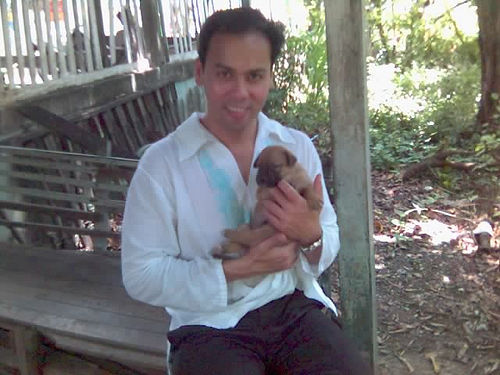
\includegraphics[width=0.4\textwidth]{src/images/2008_000026.jpg} &
        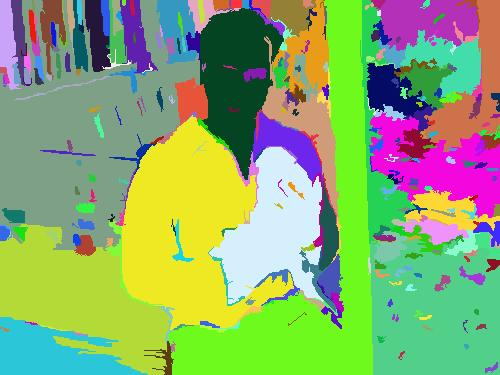
\includegraphics[width=0.4\textwidth]{src/images/2008_000026_output.jpg}
    \end{tabular}
    \caption{一张关于人的图像和它的分割结果(2008\_000026.jpg)}
    \label{figure_person}
\end{figure}

\begin{figure}[h!]
    \centering
    \begin{tabular}{cc}
        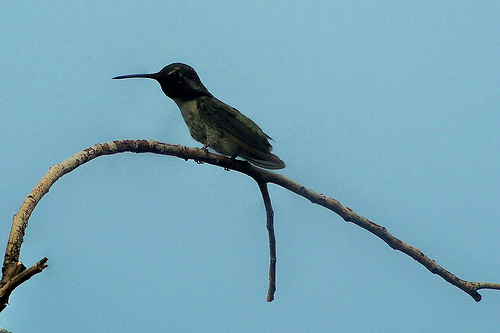
\includegraphics[width=0.4\textwidth]{src/images/2008_000123.jpg} &
        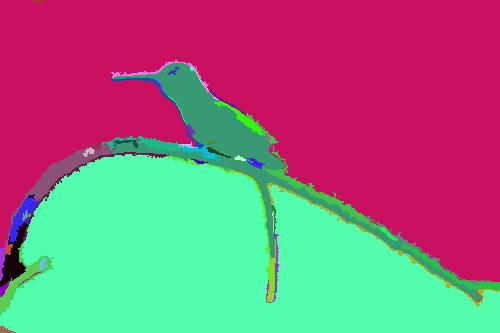
\includegraphics[width=0.4\textwidth]{src/images/2008_000123_output.jpg}
    \end{tabular}
    \caption{一张关于鸟的图像和它的分割结果(2008\_000123.jpg)}
    \label{figure_bird}
\end{figure}

\begin{figure}[h!]
    \centering
    \begin{tabular}{cc}
        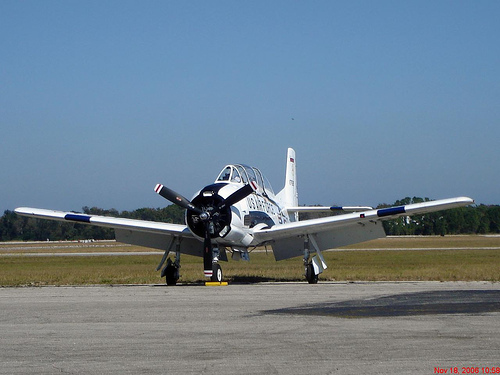
\includegraphics[width=0.4\textwidth]{src/images/2008_000021.jpg} &
        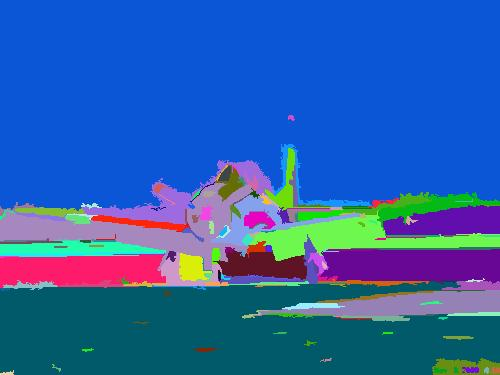
\includegraphics[width=0.4\textwidth]{src/images/2008_000021_output.jpg}
    \end{tabular}
    \caption{一张关于飞机的图像和它的分割结果(2008\_000021.jpg)}
    \label{figure_aeroplane}
\end{figure}

\begin{figure}[h!]
    \centering
    \begin{tabular}{cc}
        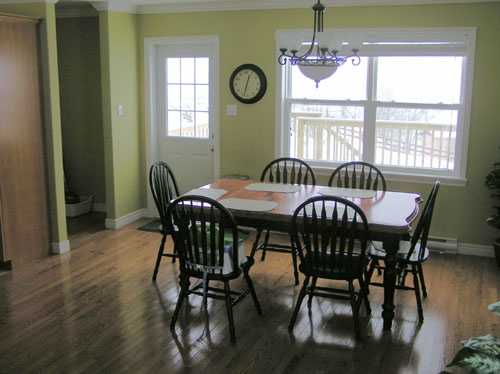
\includegraphics[width=0.4\textwidth]{src/images/2008_000043.jpg} &
        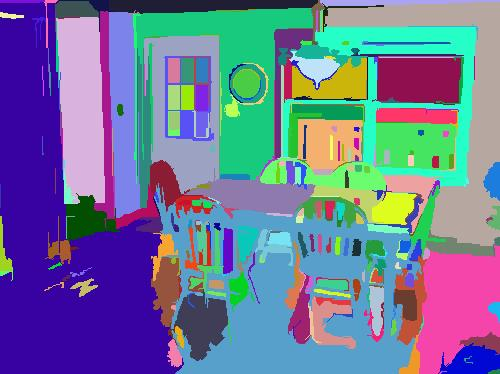
\includegraphics[width=0.4\textwidth]{src/images/2008_000043_output.jpg}
    \end{tabular}
    \caption{一张关于椅子的图像和它的分割结果(2008\_000043.jpg)}
    \label{figure_chair}
\end{figure}

% --------------------------------
\section{实验感想}

通过这次实验,熟悉了图像分割等,实现了简单的图像分割,基本达到了实验目的。


% --------------------------------
\renewcommand{\refname}{参考}
\begin{thebibliography}{9}
\bibitem{ref1} 图像分割. 维基百科. 最后修订于2015年10月20日. \url{https://zh.wikipedia.org/wiki/%E5%9B%BE%E5%83%8F%E5%88%86%E5%89%B2}
\bibitem{ref2} Visual Object Classes Challenge 2012 (VOC2012).  PASCAL2. \url{http://host.robots.ox.ac.uk/pascal/VOC/voc2012/index.html}
\end{thebibliography}

\end{document}
